\documentclass[10pt,letterpaper]{article}
\usepackage[utf8]{inputenc}
\usepackage{amsmath}
\usepackage{amsfonts}
\usepackage{amssymb}
\usepackage{braket}
\usepackage{dsfont}
\usepackage{tcolorbox}
\usepackage{graphicx}
\usepackage{placeins}
\usepackage[a4paper, margin=1in]{geometry}


\newcommand{\red}{\color{red}}
\newcommand{\blue}{\color{blue}}
\newcommand{\magenta}{\color{magenta}}
\newcommand{\black}{\color{black}}
\newcommand{\gray}{\color{gray}}

\definecolor{orange}{HTML}{FC4820}
\newcommand{\orange}{\color{orange}}

\definecolor{lblue}{HTML}{2086B0}
\newcommand{\lblue}{\color{lblue}}

\definecolor{lgreen}{HTML}{57A04D}
\newcommand{\lgreen}{\color{lgreen}}

\definecolor{dgray}{HTML}{4D4D4D}
\newcommand{\dgray}{\color{dgray}}



\def\half{{1 \over 2}}
\def\d{{\rm d}}  % Roman d for derivatives
\def\O{{\cal O}}
\def\expect#1{\left\langle #1 \right\rangle} % expectation value < >
\def\eq{Eq.~}
\def\eqs{Eqs.~}
\def\eqpar#1{(#1)} % Used to put a number in parentheses and to
                   % indicate to the renumbering program that it
                   % is an equation number.
\def\ds{\displaystyle}
\def\underarrow#1{\mathrel{\mathop{\Longrightarrow}\limits_{#1}}}
\def\implies{\quad \Longrightarrow \quad}
\def\Tr{\mathop{\rm Tr}}
\def\intinf{\int_{-\infty}^{\infty}}
\def\diag{\mathop{\rm diag}\nolimits}
\def\min{{\rm min}}


\title{Numerical Calculation of the Peak Density Integral in two Squared-Gaussian Fields}

\begin{document}
\maketitle

\section{Background}

In a series of three write-ups FIXME CITE, Professor Guth (and earlier, Saarik Kalia) has written down an integral formulation of the expected spatial number density of stationary points (and later, of minima) in a sum-of-squares gaussian field ($\Phi = \phi_1^2 + \phi_2^2$). Some of the tactics employed are similar to those used by BBKS to count minima in a single gaussian field (FIXME cite bbks). To count minima over one field configuration, one can employ \ref{eq:stationary_schematic}. This  integrand contains a delta function in the gradient of $\Phi$ to locate stationary points and a factor of the determinant of the hessian matrix of $\Phi$ to compensate for the Jacobian factor from the delta-gradient integration. Cancelling out the Jacobian forces the delta function to contribute a value of $\pm 1$ whenever the gradient-delta fires at a stationary point. The factor in the integrand of \ref{eq:stationary_schematic} which allows minima to be isolated from stationary points is the heaviside function, $\theta_H(\lambda_3^\Phi)$. $\lambda_3^{\phi}$ is the smallest eigenvalue of the hessian matrix, and can be considered an eigenvalue of curvature. Its positivity guarantees that all curvatures are ``concave up'', and the point is indeed a minimum. \ref{eq:stationary_schematic} is refined repeatedly in (Fixme writeups), but we will highlight only two central steps here. The first is a rotation in field-space, which will remain an important method as the number of fields is increased. Considering $\phi_1$ and $\phi_2$ as  coeffiecients of a pair of orthonormal basis vectors in a plane, the expression $\Phi = \phi_1^2 + \phi_2^2$ is clearly invariant under rotations in this plane, as it is simply the norm-squared of the corresponding vector. Consequently, the fields can be rotated so that only $\bar{\phi}_1$ is non-zero. Eventually, we will want to calculate the expected number density of peaks over all possible field configurations corresponding to a particular power spectrum, and so the spatial integrals in \ref{eq:stationary_schematic} will be replaced with integrals over all relevant field parameters (considering the integrand as a spatial density).The ensemble of field configurations is invariant under a rotation in field space, so when we take the expectation over all field configurations, we may consider the rotated fields as the fundamental fields ref writeup stationary). As a result, $\bar{\phi}_i \rightarrow \phi_i$, and $\phi_2 \rightarrow 0$, significantly simplifying our expression (though the gradient of $\phi_2$ is not generally zero, and will play a role in the calculation of the hessian matrix of $\Phi$. 

\begin{equation}\label{eq:stationary_schematic}
N = \int_{\cal R} \d^3 x \, \delta^3 (\partial_i \Phi ) \det
     (\partial_i \partial_j \Phi ) \, \theta_H(\lambda_3^\Phi)
\end{equation}



\par Once the field-expectation integral is set up, the next step is to change variables from the cartesian parameterization of the hessian matrix into its diagonal parameterization. This change of variables allows us to explicity enforce the positivity of the $\lambda_i$ in the limits of integration (restricting us to field minima). The rotation matrices have jacobian 1, and are parameterized by three euler angles. The euler angles integrate out trivially to prefactors, and we find ourselves left with integrals in $\lambda_1$, $\lambda_2$, and $\lambda_3$ (as well as integrals over the gradient components of $\phi_2$). We will integrate over the positive octant of the $\lambda$ space, preserving the eigenvalue ordering.
\par The integral has been boiled down to the value of $\phi_1$ (written as a deviation of $\nu$ standard deviations away from a zero field mean: $\phi_1 = \nu \sigma_0$), the three hessian eigenvalues $\lambda_i$, and the three gradient components of $\phi_2$: $\eta_i$. Our fields are gaussian, so the joint pdf of the 6 free parameters is a multivariate gaussian with covariance matrix calculated in detail in FIXME cite. Putting all of this together yields the following formula from FIXME cite.

\begin{gather} \label{eq:allspace_integral}
\begin{split}
\expect{X}_{Q_2} &= \frac{\displaystyle 30,375 \sigma_0^6}{\displaystyle 16 \sqrt{30} \pi^{5/2} \kappa^5 \sigma_1^{15}e^{-\nu^2/2} \sqrt{\kappa^2-1}} \times \int_{-\infty}^{\infty} \d \lambda_1 
     \int_{-\infty}^{\lambda_1} \d \lambda_2 
     \int_{-\infty}^{\lambda_2} \d \lambda_3 (\lambda_1 -
     \lambda_2) (\lambda_1 - \lambda_3) (\lambda_2 - \lambda_3) \\
     &\qquad \times \intinf \d \eta_{3} 
     \intinf \d \eta_{2} 
     \intinf \d \eta_{1} \,  X \, e^{- Q_2} \nonumber
\end{split}
\end{gather}


Where:
\begin{equation} \label{eq:Q2}
\begin{split}
Q_2 &= \half \nu^2 + {3 \over 2 \sigma_1^2} \sum_{i} \eta_{i}^2 \nonumber \\
     &\qquad + {5 \sigma_0^2 \over 4 \kappa^2 \sigma_1^4} \left[3
     \left( \sum_i \lambda_i^2 - {2 \over \nu \sigma_0} \sum_i
     \lambda_i  n_i^2 + {1 \over \nu^2 \sigma_0^2} \left(
     \sum_i \eta_i^2 \right)^2\right) - \left(\sum_i
     \lambda_i - {1 \over \nu \sigma_0} \sum_i \eta_i^2
     \right)^2\right] \nonumber \\ 
     &\qquad + {1 \over 2 \sigma_0^2 (\kappa^2 - 1)}
     \left[\nu \sigma_0 + {\sigma_0^2 \over \sigma_1^2}
     \left(\sum_i \lambda_i - {1 \over \nu \sigma_0} \sum_i
     \eta_i^2 \right)\right]^2 \\
\end{split}
\end{equation}


In \ref{eq:allspace_integral}, the integral is taken over $\mathbb{R}^3$ in $\eta$, but is taken over an ordered subspace of $\mathbb{R}^3$ in $\lambda$. This is an enforcement of the restriction:

\begin{equation} \label{eq:ordering}
\lambda_1 \geq \lambda_2 \geq \lambda_3
\end{equation}

Only after choosing such an ordering of eigenvalues can one guarantee unique``diagonal'' decomposition of the hessian into a product of $SO(3)$ matrices and eigenvalues. Without this ordering in place, there is a multiplicity factor of $\frac{1}{3!}$ that appears in front of the integral.

\section{Attempts at an Analytic Solution}

\subsection{Multivariate Gaussian Integrals}

Ideally, we would like to find a fully analytic solution to this integral. Its form is reminiscent of a gaussian integral in multiple variables. Such integrals are actually quite simple to evaluate analytically. Consider the following:

\begin{equation} \label{eq:multigaus}
\int_{\mathbb{R}^N} \d^N x \hspace{0.2pc} \exp \left(-\dfrac{1}{2} \hspace{0.2pc}\vec{x}^\top  \operatorname{\Sigma^{-1}} \vec{x} \right)
\end{equation}

If we want this integral to converge, $\Sigma^{-1}$ must be positive-definite, which is guaranteed if $\Sigma$ is a covariance matrix because its eigenvalues are auto-variances of the eigenvectors, and are therefore greater than zero. The inner product of $\vec{x}$ through $\Sigma^{-1}$: $\vec{x}^\top \Sigma^{-1} \vec{x}$, yields a quadratic polynomial homogeneous in $x_i$, which is exactly what we need for a general multivariate gaussian. Untangling this polynomial appears to be a particularly horrible task, but the trick is to diagonalize.
$\Sigma$ is a symmetric matrix, so its inverse must be as well:

\begin{gather*}
(\operatorname{\Sigma} \operatorname{\Sigma^{-1}})^\top = \mathds{1} \\
(\operatorname{\Sigma^{-1}})^\top \operatorname{\Sigma} = \mathds{1} \\
\therefore \hspace{1pc}  (\operatorname{\Sigma^{-1}})^\top = \operatorname{\Sigma^{-1}}
\end{gather*}

the (real) spectral theorem tells us that the diagonal decomposition:

\begin{equation} \label{eq:diagdecomp}
\operatorname{\Sigma^{-1}} = \operatorname{R^\top} \operatorname{D} \operatorname{R}
\end{equation} 

yields $R$ from $O(N)$ (the orthogonal group in $N$ dimensions).
Furthermore, a covariance matrix and its inverse are both positive-definite (to see this, invert in the eigenbasis, where the matrix is diagonal with all entries positive), so $D= D^{1/2} D^{1/2}$ with all entries real.
We may change variables:

\begin{equation} \label{eq:changevar}
\vec{x} \rightarrow \vec{u} = \operatorname{D^{1/2}} \operatorname{R} \vec{x}
\end{equation}

And now \ref{eq:multigaus} becomes:

\begin{equation} \label{eq:multigaus_trans}
\dfrac{1}{|\operatorname{\Sigma^{-1}}|^{1/2}} \int_{\mathbb{R}^N} \d^N u \hspace{0.2pc} \exp \left(-\dfrac{1}{2} \hspace{0.2pc} \vec{u}^\top \vec{u}\right)
\end{equation}

Where the determinant prefactor comes from the jacobian of our change-of-variables. Re-writing \ref{eq:multigaus_trans}:

\begin{equation} \label{eq:multigaus_trans}
\dfrac{1}{|\operatorname{\Sigma^{-1}}|^{1/2}} \prod_{i=1}^{N} \int_{\mathbb{R}} \d u_{i} \hspace{0.2pc} \exp\left(-\dfrac{1}{2} \hspace{0.2pc} u_{i}^2\right)
\end{equation}

Performing the canonical integration:

\begin{equation} \label{eq:multigaus_final}
\dfrac{1}{|\operatorname{\Sigma^{-1}}|^{1/2}} \prod_{i=1}^{N} \int_{\mathbb{R}} \d u_{i} \hspace{0.2pc} \exp \left(-\dfrac{1}{2} \hspace{0.2pc} u_{i}^2 \right) = (2\pi)^{N/2} \hspace{0.2pc}|\operatorname{\Sigma}|^{1/2}
\end{equation}

Polynomial prefactors of the exponent can be obtained by parameter-differentiation, so this technique is quite general. 

The remaining complication is an inhomogeneous polynomial in the exponent. To order 2, this means there may be linear terms. There is a nice trick (variable change) to address this case. What follows is an adaptation of FIXME Cite.

Say we encounter the following integral:

\begin{equation} \label{eq:multigaus_linterm}
\int_{\mathbb{R}^N} \d^N x \hspace{0.2pc} \exp \left(-\dfrac{1}{2} \hspace{0.2pc}  \vec{x}^\top \operatorname{\Sigma^{-1}} \vec{x} + \vec{J}^\top \vec{x} \right)
\end{equation}

Which has linear terms: $\vec{J}^\top \vec{X}$. The trick is the change of variables:

$$\vec{x} = \operatorname{\Sigma} \vec{J} + \vec{\tilde{x}}$$

The integral becomes, after this transformation:

\begin{equation} \label{eq:multigaus_lintrick}
\exp\left(\dfrac{1}{2}\vec{J}^\top \operatorname{\Sigma} J\right) \int_{\mathbb{R}^N} \d^N \tilde{x} \hspace{0.2pc} \exp\left(-\dfrac{1}{2} \hspace{0.2pc} \vec{\tilde{x}}^\top \operatorname{\Sigma^{-1}} \vec{\tilde{x}} + {\vec{J}}^\top \vec{\tilde{x}}\right)
\end{equation}

The new integrand has a homogeneous polynomial in its exponent, and will therefore yield to the same diagonalization technique as \ref{eq:multigaus}.

\section{Lambdas First} \label{lambdasec}

With these techniques in hand, let us examine our density integral, ~\ref{eq:allspace_integral} and it's exponenet, ~\ref{eq:Q2}. The first thing to notice is that $Q_2$ is quadratic in $\lambda$, but quartic in $\eta$. Since the gaussian tricks above do not apply to a quartic polynomial, there is no obvious way to proceed in 6 dimensions. This roadblock suggests that we try one of the 3 dimensional subspaces (one accorded to the the three $\lambda_i$ and the other to the three $\eta_i$), treating variables from the other as constants. Since the $\lambda_i$ only appear to order 2, we will start there. Treating the $\eta_i$ as constants, $Q_2$ is an inhomogeneous polynomial of order 2 in $\eta$, and so should be vulnerable to the diagonal separation technique described above.
\par Indeed, it is possible to diagonalize the matrix which generates this polynomial, and to change variables accordingly. Unfortunately, we are only interested in field minima, and so our $\lambda$ integrals are not taken over all space. To simplify the limits of integration, we can forget the ordering of $\lambda_i$ and simply integrate each $\lambda$ over $[0,\infty)$, remembering to include the $1/3!$ prefactor. If we were integrating in only one $\lambda$ dimension, we could cast the integral as an evaluation of the gamma function:

\begin{equation} \label{eq:gamma}
\Gamma(t) = \int_{0}^{\infty} x^{t-1} e^{-x} \d x
\end{equation}

Unfortunately, because of the linear terms (a constant vector shift as variable change: \ref{eq:changevar}) and the diagonalization rotation, the limits of integration are no longer simple, even neglecting the $\lambda$ ordering. Call the new variables $u_1$, $u_2$, and $u_3$, in which the polynomial exponent becomes $-\frac{1}{2}(u_1^2 + u_2^2 + u_3^2)$. The limits of integration, even without linear terms, define a paralellpiped in 3-space which is bounded on three faces, and extends infinitely to cover what a distorted image (non-$O(3)$ linear mapping) of the positive  $\lambda$ octant. The issue is, while $R$ may be an orthogonal operator, $D^{1/2}R$ is not, so the limits of integration of $u_3$ will be a linear function of $u_1$ and $u_2$. $u_2$ will be a linear function of $u_1$, and $u_1$ will be free. Put in more geometric terms, the planes which bound this parallelpiped are not orthogonally oriented. Now that the limits of the innermost integral are no longer $0$ and $\infty$, there is no gamma-function trick available.  The innermost integral yields an error function in the next two variables. One integral can be done, as the integrals of $e^{-x^2}$ can be expressed in terms of error functions:

\begin{equation} \label{eq:erfint}
\int \d u_1 \hspace{0.2pc}  \text{erf}(u_1) = \frac{e^{-u_1^2}}{\sqrt{\pi}} + u_1  \hspace{0.2pc}  \text{erf}(u_1)
\end{equation}

And the diagonalized integrand can be expressed as the product: $\exp(-\frac{1}{2} u_1^2) \exp(-\frac{1}{2} u_2^2) \exp(-\frac{1}{2} u_3^2)$, so the integral can be partially factored:

\begin{equation} \label{eq:gausnest}
A \int_{D1} \d u_1 \exp(-\frac{1}{2} u_1^2) \int_{D2(u_1)} \d u_2 \exp(-\frac{1}{2} u_2^2) \int_{D3(u_1,u_2)} \d u_3 \exp(-\frac{1}{2} u_3^2)
\end{equation}

Where $A$ is a prefactor depending only on $\eta$ and $\nu$, and $D1$,$D2$,$D3$ are domains of integration whose cartesian product corresponds to the parallelpiped volume, with $D2(u_1)$ a function of $u_1$, and $D3(u_1,u_2)$ a funtion of $u_1$ and $u_2$. These domains should be half-infinite, with either upper or lower bounds, depending on the nature of the variable transofrmation. We will call the finite bounds $l_3(u_1,u_2)$, $l_2(u_1)$, and $l_1$ respectively, where $l_i()$ is an affine transformation of its input vector (linear transformation with constant offset) resulting from the origin-shifts and non-orthogonality of the planes partially bounding the integration parallelpiped.

We can proceed by evaluating the $u_3$ integral in \ref{eq:gausnest}. Unfortunately, evaluating the corresponding antiderivative over the half-infinite interval $D3$ yields a term of the form: 

$$\frac{e^{-l(u_1,u_2)^2}}{\sqrt{\pi}} + l(u_1,u_2) \hspace{0.2pc}  \text{erf}(l(u_1,u_2))$$ 

If we then attempt the $u_2$ integral, we need to evaluate the antiderivative: 

\begin{equation*}
\int \d u_2  \hspace{0.2pc} \exp(-\frac{1}{2} u_2^2) \left(\dfrac{e^{-l(u_1,u_2)^2}}{\sqrt{\pi}} + l(u_1,u_2) \hspace{0.2pc} \text{erf}\left(l(u_1,u_2)\right)\right)
\end{equation*}

And here we spot the cloven hoof. Even the relatively simple function:

\begin{equation} \label{eq:nonointegral}
\exp(-x^2)  \hspace{0.2pc} \text{erf}(x+c)
\end{equation}

does not appear to have an anti-derivative. Consulting a compendium of error-function integrals and antiderivatives FIXME CITE OWEN, we find expressions for similar integrals, but they must be taken over particular domains. Integrals with general boundaries (like ours) do not seem to translate into any of the special cases, although that doesn't mean there isn't a clever trick hiding somewhere in those integral tables.
It is not obvious how to proceed with the $\lambda$ integrals, so we turn to the $\eta$ integrals to see if any headway can be made there.

\subsection{Eta Integrals}

\vspace{1pc}
\begin{equation*}
\begin{split}
Q_2 &= \half \nu^2 + {3 \over 2 \sigma_1^2} \sum_{i} \eta_{i}^2 \nonumber \\
     &\qquad + {5 \sigma_0^2 \over 4 \kappa^2 \sigma_1^4} \left[3
     \left( \sum_i \lambda_i^2 - {2 \over \nu \sigma_0} \sum_i
     \lambda_i  n_i^2 + {1 \over \nu^2 \sigma_0^2} \left(
     \sum_i \eta_i^2 \right)^2\right) - \left(\sum_i
     \lambda_i - {1 \over \nu \sigma_0} \sum_i \eta_i^2
     \right)^2\right] \nonumber \\ 
     &\qquad + {1 \over 2 \sigma_0^2 (\kappa^2 - 1)}
     \left[\nu \sigma_0 + {\sigma_0^2 \over \sigma_1^2}
     \left(\sum_i \lambda_i - {1 \over \nu \sigma_0} \sum_i
     \eta_i^2 \right)\right]^2 \\
\end{split}
\end{equation*}
\vspace{1pc}


The $\eta$ integrals are both more and less friendly than the $\lambda$ integrals. On one hand, the $Q_2$ polynomial ((\ref{eq:Q2}), reprinted above for convenience) is quartic in $\eta_i$, which complicates things significantly. On the other hand, the domain of integration is all of $\mathbb{R}^3$, which suggests that diagonalization techniques might not lead to error functions, as before. Two angles of attack will be discussed here.

\subsubsection{Change of Variables}

Although $Q_2$ is quartic in $\eta_i$, there are no linear or cubic terms. Furthermore, $\eta_i$ only enters as $\eta_i^2$. Consqeuently, we may rewrite the $\eta$-dependent form of $Q_2$ in inner-product notation not in terms of $\vec{\eta}$, but rather:
$$\vec{\eta^2} = (\eta_1^2,\eta_2^2,\eta_3^2)$$.

Rewriting $Q_2$ with this handy vector yields:

\begin{equation} \label{eq:eta_squared}
Q_2 = -\frac{1}{2} \left(\vec{\eta^2}^\top \operatorname{M} \vec{\eta^2} + J^\top \vec{\eta^2} + c \right)
\end{equation}

Exploiting the representation of the $\eta_i^2$ in a vector format, we perform a change of variables.

$$v_i = \eta_i^2$$

This is a transformation, component-wise, of $\vec{\eta^2}$ into a vector $\vec{v}$.

This transformation yields the jacobian matrix:

\begin{equation}
\frac{\partial v_i}{\partial \eta_j} = 2(v_i)^{1/2} \delta^{i}_{j}
\end{equation}

Incorporating the corresponding jacobian factor, the eta integrals become:

\begin{equation} \label{eq:eta_lintrick}
\exp\left(\frac{1}{2}\vec{J}^\top \operatorname{\Sigma} J\right) \int_0^{\infty} \d v_1 \int_0^{\infty} \d v_2 \int_0^{\infty} \d v_3 \hspace{0.5pc}  (64 v_1 v_2 v_3)^{-1/2} \exp\left(-\frac{1}{2} \vec{v}^\top \operatorname{\Sigma^{-1}} \vec{v} + \vec{J}^\top \vec{v}\right)
\end{equation}

To remove the term linear in $v_i$, we use the trick we applied to \ref{eq:multigaus_linterm}:

$$\vec{v} = \operatorname{M^{-1}} \vec{J} + \vec{\tilde{v}}$$

Which substitution yields:

\begin{gather} 
\exp\left(\frac{1}{2} \hspace{0.2pc} \vec{J}^\top \operatorname{M}^{-1} J\right) \int_{-w_1}^{\infty} \d \tilde{v_1} \int_{-w_2}^{\infty} \d \tilde{v_2} \int_{-w_3}^{\infty} \d \tilde{v_3}   \hspace{0.2pc} (64 (\tilde{v}_1 + w_1)(\tilde{v}_2 + w_2)(\tilde{v}_2 + w_2))^{-1/2} \nonumber \\ 
\times \exp\left(-\frac{1}{2} \hspace{0.2pc} \vec{\tilde{v}}^\top 			\operatorname{M} \vec{\tilde{v}} + \vec{J}^\top \vec{\tilde{v}}\right) \\ \nonumber
\end{gather}

Where $w_i = {(\operatorname{M}^{-1})_i}^j J_j$
\vspace{1pc}

In preparing our integral for diagonalization, we have fallen into the same nested-erf trap as in Section \ref{lambdasec}! The change of variables to $v_i = \eta_i^2$ changed the limits of integration to half-lines. As a result, diagonalization will scramble the limits, yielding the same kind of parallelpiped trouble as before.

As a last-ditch attempt to salvage this integration technique, one might consider the $64 (\tilde{v}_1 + w_1)(\tilde{v}_2 + w_2)(\tilde{v}_2 + w_2))^{-1/2}$ factor as a handle for contour integration in the complex plane. Unfortunately, although this jacobian factor does have singularities in each $\tilde{v}_i$ plane, and the complementary factor is an entire function, these singularities are not poles, but rather boundaries of branch cuts. Without any poles, it does not appear to be possible to leverage the residue theorem.

\subsubsection{Multilinear Forms}

In our efforts to write order 2 polynomials as inner products of vectors across some $\Sigma^{-1}$ matrix, we have been making implicit use of a bijective relationship between quadratic homogeneous (all terms have the same total order: 2) polynomials in $n$ variables and inner products of the form: $\vec{x}^\top \operatorname{\Sigma}^{-1} \vec{x}$ where $\operatorname{\Sigma}^{-1}$ is a symmetric matrix. Such matrices, in this context, are representations of a map of a product of vector spaces onto their underlying field: $F: V \times V \rightarrow \mathbb{R}$ (the reals, in our case). The motivation for this point of view is that it can be generalized to multi-linear forms, which are capable of mapping tensor products of more than two vector spaces onto homogeneous polynomials of arbitrary degree. These multi-linear forms have representation as tensors, and in the case of symmetric tensors, there is, once again, a bijection between homogeneous polynomials of degree $k$ and symmetric tensors of order $k$ (where the order of such a tensor is the number of vector-space factors in the cartesian product: $V^{\times k}$ which is mapped to $\mathbb{R}$). The connection is made clearer when these tensors are used as multilinear forms to map elements of the vector space: $V^{\times k}$ onto $\mathbb{R}$. To visualize the generalization, let's begin with the order-2 (the matrix case).

Let $\mathcal{P}_2(x)$ be a homogeneous polynomial of order 2, where $x\in V_2(\mathbb{R})$, which is to say x is a vector in a real vector space of dimension $2$.

Generally:

$$ \mathcal{P}_2(x) =  \alpha x_1^2 + \beta x_1 x_2 + \gamma x_2^2 $$

The standard (euclidean) inner product, which is a bilinear form represented here as the identity on $V_2(\mathbb{R})$, will produce the following polynomial:

$$ \sum_{i,j} \mathds{1}_{ij} x_i x_j = x_1^2 + x_2^2$$

So, if we want to be able to generate cross-terms, and to apply to each term an arbitrary prefactor (to produce more general polynomials), we need to replace $\mathds{1}$ with a more general matrix. In this case, to generate any $\mathcal{P}_2(x)$, we can use the matrix:


\[M = \left(\begin{array}{ccc}
\alpha & \beta/2 \\
\beta/2 & \gamma \\
\end{array} \right)\] 

Employing $M$ as a bilinear form, we find:

\begin{equation} \label{eq:bilinear_form}
\mathcal{P}_2(x) =  \sum_{i,j} M_{ij} x_i x_j = \alpha x_1^2 + \beta x_1 x_2 + \gamma x_2^2 
\end{equation}


What if we want to work with higher-degree polynomials (as in the quartic $\eta$ case)?
The above correspondence suggests a relationship between symmetric multilinear forms (represented as order-$k$ tensors) and homogeneous polynomials of degree $k$. Indeed, there is a bijection between these two classes of mathematical objects (FIXME CITE SYMMETRIC):

\begin{equation} \label{eq:multilinear_form}
\mathcal{P}_k(x) =  \sum_{i_1...i_k} M_{i_1...i_k} x^{i_1}...x^{i_k}
\end{equation}

Where the requirement that $M$ is a symmetric tensor translates into the statement that M, represented in some set of indices, is invariant under a permutation of a particular index-vector:

$$ M_{i_1...i_k} = M_{\sigma(i_1,...,i_k)}$$

Where $\sigma()$ is any element of the permutation group of $k$ elements.

Which is an elegant formulation, but what is the application to our $\eta$ integration?

We were able to decouple the integrals in the gaussian case by diagonalizing the matrix representation of a symmetric bilinear form, $\Sigma^{-1}$ (\ref{eq:multigaus}) and changing variables accordingly, might it be possible to ``diagonalize'' the tensor representation of the quartic form in $\eta$ and change variables in the $\eta$ vector space to decouple the integral into a product of integrals, each of which could perhaps be turned into an evaluation of the gamma function?

Let us, for the time being, neglect the inhomogeneous terms in the $Q_2$ polynomial (it may be possible to perform a trick like that which was done in the gaussian case to kill the linear terms), and consider the homogeneous case.

As it happens, symmetric tensors do admit a ``diagonal'' decomposition, sometimes called the \textit{Waring decomposition}. Let $T$ be a tensor of order $k$, then there exist $v_i\in V_k(\mathbb{R})$ such that:

\begin{equation} \label{eq:waring}
T = \sum_{i=1}^r \lambda_i v_i^{\otimes k}
\end{equation} 

This is, essentially, an eigenvalue/eigen-(rank-1)tensor decomposition.

Recall that our homogeneous polynomial, $\mathcal{P}_4(\eta)$ has representation:

\begin{equation} \label{eq:etaform}
\mathcal{P}_4(\eta) =  \sum_{i_1...i_k} T_{i_1...i_k} \eta^{i_1}...\eta^{i_k}
\end{equation}

$T$ is symmetric and order-$4$, so this can be written:

\begin{equation} \label{eq:etaform_eigen}
\mathcal{P}_4(\eta) =  \sum_{i_1...i_k} \left(\sum_{\alpha=1}^r \lambda_{\alpha} v_{\alpha}^{\otimes k}\right)_{i_1...i_k} \eta^{i_1}...\eta^{i_k}
\end{equation}

As a reminder, $i_l$ is the $l$th index of both the $\eta$ tensor we're contracting with $T$, and the $v_i^{\otimes k}$ eigentensor of $T$. But, because both the $\eta$ and $v$ tensors are k-th tensor products of a single vector, $\eta$ and $v_i$ respectively, they have simple forms in index notation:

\begin{gather*}
\left(\eta^{\otimes k}\right)^{i_1...i_k} = \eta^{i_1}...\eta^{i_k} \\ 
\left(v_{\alpha}^{\otimes k}\right)^{i_1...i_k} = v_{\alpha}^{i_1}...v_{\alpha}^{i_k} \\
\end{gather*}

So we may rewrite \ref{eq:etaform_eigen}, exchanging summations:

\begin{equation} \label{eq:etaform_eigen}
\mathcal{P}_4(\eta) =  \sum_{\alpha=1}^r \lambda_{\alpha} \sum_{i_1...i_k} \left(v_{\alpha}\right)_{i_1}...\left(v_{\alpha}\right)_{i_k} \eta^{i_1}...\eta^{i_k}
\end{equation}

Notice that the innermost summand is simply a power of inner products!
Exploiting a combination of standard and Einstein summation notations:


\begin{equation} \label{eq:etaform_eigen_niii}
\mathcal{P}_4(\eta) =  \sum_{\alpha=1}^r \lambda_{\alpha} \left(\left(v_{\alpha}\right)_i\eta^i\right)^4
\end{equation}

And this can be written in the form:

\begin{equation} \label{eq:etaform_eigen_niii}
\mathcal{P}_4(\eta) =  \delta_{\alpha \beta \gamma \delta} \left(\left(\Lambda^{1/4}\right)^{\alpha}_{j} W^{j}_i\eta^i\right)\left(\left(\Lambda^{1/4}\right)^{\beta}_{j} W^{j}_i\eta^i\right)\left(\left(\Lambda^{1/4}\right)^{\gamma}_{j} W^{j}_i\eta^i\right)\left(\left(\Lambda^{1/4}\right)^{\delta}_{j} W^{j}_i\eta^i\right)
\end{equation}

Where:

\[W = \left(\begin{array}{c}
\vec{v_1} \\
\vec{v_2} \\
\vec{v_3} \\
\vec{v_4} \\
\end{array} \right)\] 

And

\[\Lambda = \left(\begin{array}{cccc}
\lambda_1 & 0 & 0 & 0 \\
0 & \lambda_2 & 0 & 0 \\
0 & 0 &\lambda_3 & 0 \\
0 & 0 & 0 & \lambda_4 \\
\end{array} \right)\] 


Finally, we have arrived at our diagonal destination. With the variable change:

$$ \vec{u} = \Lambda^{1/4} W \vec{\eta} $$

The polynomial $\mathcal{P}_4(\eta)$ becomes:

\begin{equation} \label{eq:etaform_eigen_niii}
\mathcal{P}_4(\eta) =  \delta_{\alpha \beta \gamma \delta} u^{\alpha} u^{\beta} u^{\gamma} u^{\delta} = u_1^4 + u_2^4 + u_3^4 + u_4^4
\end{equation}

This appears to be cause for celebration, as the integral would now be seperable, and (crucially) the limits are still full real lines for each $\eta$, so the variable change will not introduce any of this parallelogram nonsense. However, there are two snags which I have not overcome.

The first is the question of how to remove the quadratic terms to homogenize this polynomial. I have some ideas, but have not yet been able to clarify the procedure (it might not be do-able: this needs investigation).

The second snag is more fundamental, and, if solvable, will require serious mathematical gymnastics.

Earlier, when introducing the Waring tensor decomposition \ref{eq:waring}, I slipped something under the radar. In the order-2 case, the waring decomposition for a real symmetric tensor is the diagonal decomposition for a real symmetric matrix. We are guaranteed that the number of eigen-tensors in the decomposition sum (tensor products of the eigen-vectors in the matrix case, call this number $r$) is exactly equal to the dimension of the underlying vector space ($k$).

This decomposition, in tensor notation, looks like this:

\begin{equation} \label{eq:waring-o2}
T = \sum_{i=1}^d \lambda_i v_i^{\otimes 2}
\end{equation} 

Where $v_i \in V_d(\mathbb{R})$.

But the crucial difference between this special case and the Waring decomposition is that $r=d$. There are never more terms in the decomposition than there are dimensions in the underlying vector space $V_d(\mathbb{R})$. However, in higher-order decompositions, the rule is: $r\geq d$. And if there are more terms in the decomposition than there are dimensions in the vector space: A) the $v_i$ cannot be linearly independent, and B) we cannot write down $W$ as a 3-by-3 matrix. It would appear that we need another $\eta$ dimension to effect the change of variables. I don't know if it's possible to embed our $\eta$ integral in a higher dimensional integral and then extract the 3-d integral after the fact.

Unfortunately, I think this isn't possible (though this needs to be checked), because building the $W$ matrix out of linearly dependent rows will cause it to have a rank less than $r$, which, in an $r$ by $r$ matrix, implies determinant zero, and the change of variables is not invertible, and therefore invalid. Although, it is possible that in some higher dimensional space, $r=d$, and the construction is valid.

 Furthermore, in the order-2 case, the real spectral theorem guarantees that these vectors are mutually orthogonal, so that the $W$ matrix is an orthogonal operator. It is not obvious to me that, even if $r=d$, there is still a spectral theorem for these decompositions. The jacobian of the transformation will therefore introduce a nasty function of the $u_i$ in front of the exponential. 

 Moving forward along this line of thinking will probably require a thorough literature search, beginning with FIXME REF SYMMETRIC.











%\ref{eq:etaform_eigen} has an evil look about it, so let's consider the order-2 (matrix) case:

%\begin{equation} \label{eq:etaform_o2}
%\mathcal{P}_4(\eta) =  \sum_{\alpha=1}^r \lambda_{\alpha} \sum_{i_1,i_2} \left(v_{\alpha}\right)_{i_1}%%%\left(v_{\alpha}\right)_{i_2} \eta^{i_1}eta^{i_2}
%\end{equation}

%Writing this in Dirac notation, we see a familiar face of the eigen-decomposition!


%\begin{equation} \label{eq:etaform_dirac}
%\sum_{\alpha=1}^r \lambda_{\alpha} \sum_{i_1,i_2} \left(v_{\alpha}\right)_{i_1}\left(v_{\alpha}\right)_{i_2} %\eta^{i_1}\eta^{i_2} = \bra{\eta} \left(\sum_{\alpha=1}^r \ket{v_{\alpha}} \lambda_{\alpha} \bra{v_\alpha} %\right) \ket{\eta} = \bra{\eta} T \ket{\eta}
%\end{equation}

%The analogy to the order-2 case guides our next step. 

\section{A Numerical Solution} \label{numsol}

\subsection{Monte Carlo Integration}

It appears that (for now), analytic integration of either 3-space ($\vec{\eta}$ or $\vec{\lambda}$) is intractable. Instead, we will resort to numerical integration. In roughly 1 to 3 dimensions, the way to integrate is with quadrature rules treating the N-volume integral as N integrals over intervals of the real line. Unfortunately, the errors from these approximation methods, though manageable in one or two dimensions, increase rapidly with the number of layers in this nested integral. To compute multi-dimensional integrals (6, in our case) to a specified error tolerance in a reasonable amount of time requires an altogether different approach.

The technique we will explore is called monte-carlo integration, and it exploits the law of large numbers.
Stated without much rigor, the law of large numbers relates sample averages of draws from a random distribution to its expected value.

Let:

$$\bar{X} = \displaystyle{\frac{1}{N}} \sum_{i=1}^N X_i$$

be the sample average, where $X_i$ are samples of a random variable $x$ disributed according to some distribution with pdf $f(x)$.

If this pdf is well behaved (integrable, for our intents and purposes), then we may also define the expectation value:

$$\lbrace x \rbrace = \int_{D} \d x x f(x)$$

Where $D$ is the domain in which $f(x)$ is supported.

The law of large numbers says (roughly) that $\bar{x} \rightarrow \langle x \rangle$ as $N \rightarrow \infty$.

Now, this law also applies to expectation values of functions of a random variable, so that:

\begin{equation} \label{eq:largen_func}
\displaystyle{\frac{1}{N}} \sum_{i=1}^N g(X_i) \rightarrow \int_{D} \d x g(x) f(x) | N \rightarrow \infty
\end{equation}

This suggests that we can approximate the integral $\int_{D} \d x g(x) f(x)$ by drawing samples $X_i$ from a distribution $f(x)$, calculating $g(X_i)$, and summing the results. This approximation is the essence of monte carlo integration.

Of course, such an approximation is not terribly useful without an error estimate. We may approximate the standard error on the mean (which will be the standard error in our approximation of the expected value by the sample averate) by: $s_g / \sqrt{N}$, where $s_g$ is an unbiased estimate of the standard deviation of $g(x)$: $\sigma_g$, using our $N$ samples $g(X_i)$.
Three things happen as N becomes large. The first, which is a consequence of the law of large numbers, is that $s_g \rightarrow \sigma_g$, so our approximation of the standard error approaches the true standard error.
The second allows an interpretation of the standard error according to a normal distribution. This is where the central limit theorem comes into play. Again, provided with neither proof nor rigorous language, this theorem states that the distribution of the arithmetic mean of an arbitrary number of independent samples of an arbitrary distribution will approach a normal distribution as the number of samples becomes large. This allows us to interpret the standard error in a statistical sense: ``If  we repeat our monte carlo integration a large number of times, we expect the true value of the integral to lie within $\pm \sigma_g$ of our approximation in roughly 68\% percent of trials''
The third effect, which is immediately obvious, is that the standard error (which we now see is not a strict upper bound on the error, but rather a statistical bound) decreases as $1/\sqrt{N}$.
This decreasing error is the true strength of monte carlo methods. While quadrature methods (with strict error bounds) may exhibit errors that decrease more quickly with N (the number of iterations) in few dimensions, the decrease becomes slower and slower in more dimensions. The monte carlo scaling, on the other hand, does not depend on the number of dimensions, and is therefore ideal for many-dimensional integration (although the error bound could still be terrible in an absolute sense, if $\sigma_g$ is large, this does not impact the scaling w/r/t $N$).

\subsection{The Metropolis Method}

FIXME add a moving tale of hope, disappointment, and loss w/r/t the Metropolis method.


\subsection{The Vegas Algorithm}
\par Naively, if we wanted to do a monte carlo integration in an arbitrary number of dimensions ($N$) on the following integral:

$$\int_{D} \d^N x g(\vec{x})$$

We would simply draw $X_i$ from the uniform distribution over $D$. This is a simple approach, but it may take a long time to reach some desired error tolerance beacuse $\sigma_g$ could be large, requiring large $N$ to compensate. Intuitively, we can imagine a bumpy surface (to keep it simple, imagine a scalar surface over a two dimensional domain) and a process for picking points over its domain. Each time a point is picked, it is evaluated, resulting in a little dot on the surface at that value. If we pick points with equal frequency in the valleys and the mountains of this surface, we are, in a sense wasting time. The valleys will contribute little to the sum, so we would be better served by picking points in regions of our domain that support mountains more frequently than in those that support valleys. There are two ways to achieve this, both of which are explained in (FIXME CITE NR). To these explanations I will likely not do justice, although hopefully I can provide an intuitive cartoon.

The first technique is called \textit{stratified sampling}. The idea here is to partition the sampling domain, and to assign a number of samples to each subdomain according to the variance of the function within that subdomain. Of course, the variance is usually not known ahead of time, so this technique is applied iteratively. For example, one could generate a grid partition of the domain and assign a set number of samples to each subdomain. The variance could be estimated in each subdomain by evaluating the samples, and then the size of each subdomain could be adjusted in inverse proportionality to the variance of the first step. This process is then repeated, so the subdomains tighten around mountains and broaden around valleys, minimizing the variance within each subdomain. The sum of the estimate of the function variance within each subdomain will then provide an estimate of the variance over the entire domain. By reducing the variance in each subdomain, the total variance can be minimized. (FIXME sum-of-squares argument)

The second technique is known as \textit{importance sampling}. Importance sampling is essentially a change of probability measure under the integral:

\begin{equation} \label{eq:importance}
\int_{D} \d^N x g(\vec{x}) \rightarrow \int_{D} \d^N x \displaystyle{\frac{g(\vec{x})}{f(\vec{x})}} f(\vec{x})
\end{equation}

This can then be approximated by sampling $X_i$ according to the disribution $f(x)$ and summing $\frac{g(\vec{X_i})}{f(\vec{X_i})}$. If $f(x)$ is similar in shape to $g(x)$, then the division will flatten out mountains and valleys, and reduce overall function variance, reducing $\sigma_g$. $f(x)$, of course, must be a valid, normalized pdf, and the optimal $f(x)$ is given by: $\frac{|g|}{G}$ Where G is the volume-integral of $|g|$, required for normalization (FIXME cite NR). Of course, this requires foreknowledge of a volume integral very similar to the one we're trying to find in the first place, so this form usually isn't helpful.
What can be done, without foreknowledge, is to begin by sampling uniformly from the domain supporting $g$, laying down a grid, and building a discrete approximation to the function on these grid cubes. This discrete approximation can then be normalized with a simple sum, and used to perform importance sampling on the next iteration. In this way, the discrete $f$ approximates the shape of $g$ more finely with each iteration, reducing variance.

The Vegas algorithm implements both of these techniques (though the details of the implementation are more complicated than these intuitive descriptions, for details, see (FIXME CITE NR)) to adaptively estimate an integral, reducing the variance at each iteration. The basic strategy is to run a first series of iterations on an integrand, throwing away the integral estimates, but keeping the subdomain layout and importance function estimates which are refined with each step. This is somewhat like the ``burn-in'' period for a markov chain monte carlo technique. After the variance has settled down (the exact threshold for ``settlement'' is not set in stone), one then runs another sequence, with or without adaptive iteration, and stores the weighted average of the integral estimates and the associated error estimate.

It is this algorithm that was finally chosen to attack our 6-dimensional minimum-density integral.

FIXME cite python package!

\section{Slaying the Chimera: Results from Numerical Integration} \label{results}

Ultimately, the goal of this work is to calculate the expected density of field minima: 

$$\left\langle \frac{\partial n_{2,min}}{\partial \nu} \right\rangle = \displaystyle{\frac{3 \sqrt{6} \nu e^{-\nu^2/2}}{4 \pi^{3/2} \sigma_1^3}} \expect{\lambda_1 \lambda_2 \lambda_3 \Theta(\lambda 3)}_{Q_2}$$

This integral does not appear to yield to attempts at analytic solution, so we have chosen the Vegas algorithm to approximate it numerically.

As mentioned in the descriptions of numerical integration techniques, each approach was vetted by calculation of a ``toy integral'' with an integrand similar to the full density integrand, in order to gauge performance. This toy integral is the signed number density of stationary points, which was evaluated analytically in (FIXME CITE) by Professor Guth and Saarik Kalia:

\begin{equation} \label{eq:toyint}
\expect{\lambda_1 \lambda_2 \lambda_3}_{Q_2} = \displaystyle{- \frac{\sigma_1^6 (\nu^4 - 6\nu^2 +3)}{27 \nu \sigma_0^3}}
\end{equation}

As mentioned in Section \ref{numsol}, the Vegas algorithm was the only technique which managed to produce approximations with error estimates that reliably described the true error w/r/t the analytic solution. Once it became clear that Vegas was the victor, the next order of business was to demonstrate that this integration technique was capable of producing estimates with sub-percent errors. 

The vegas algoritm was run on the toy integral with simple values of $\sigma_1=2$, $\sigma_2=2$, and $\kappa=2$ chosen not to correspond to any real power spectrum, but out of convenience. The algorithm was run with increasing sample resolutions of $10^4$, $10^5$, and $10^6$ samples per iteration, and the results are plotted in Figures \ref{fig:toy_e4_wide}, \ref{fig:toy_e5_wide}, and \ref{fig:toy_e6_wide}; respectively.

Notice that the absolute error is decaying with increasing resolution (as expected), but also that the $Chi^2_{red}$ value for $10^4$ samples per iteration is disturbingly distant from unity. This is likely a consequence of the law of large numbers as applied to the sample variance. Near $\nu$ = 0, $Q_2$ appears to vary rapidly. With few samples, the sample estimate of variance at small $\nu$ is likely underestimating the true variance, which leads to an underestimate of the error in the integral mean, which leads to a poor ``goodness of fit''. This improves with increasing numbers of samples, which is consistent with the tendency of the sample variance toward the true variance as $N \rightarrow \infty$. According to the analytic formulation of this integral (\ref{eq:toyint}), there is a singularity at $\nu=0$. Hopefully, there will be no singularities in the true density integral, so it is not profitable at this point to critique the performance of the integral at extremely small $\nu$.

\FloatBarrier

\begin{figure}[t] %The capital H inside the square brackets is what forces the image to go exactly where I've placed in in the text. You need to be using the float package for this to work. 
\centering %I've put the centering command here so that the image appears centered on the page. 
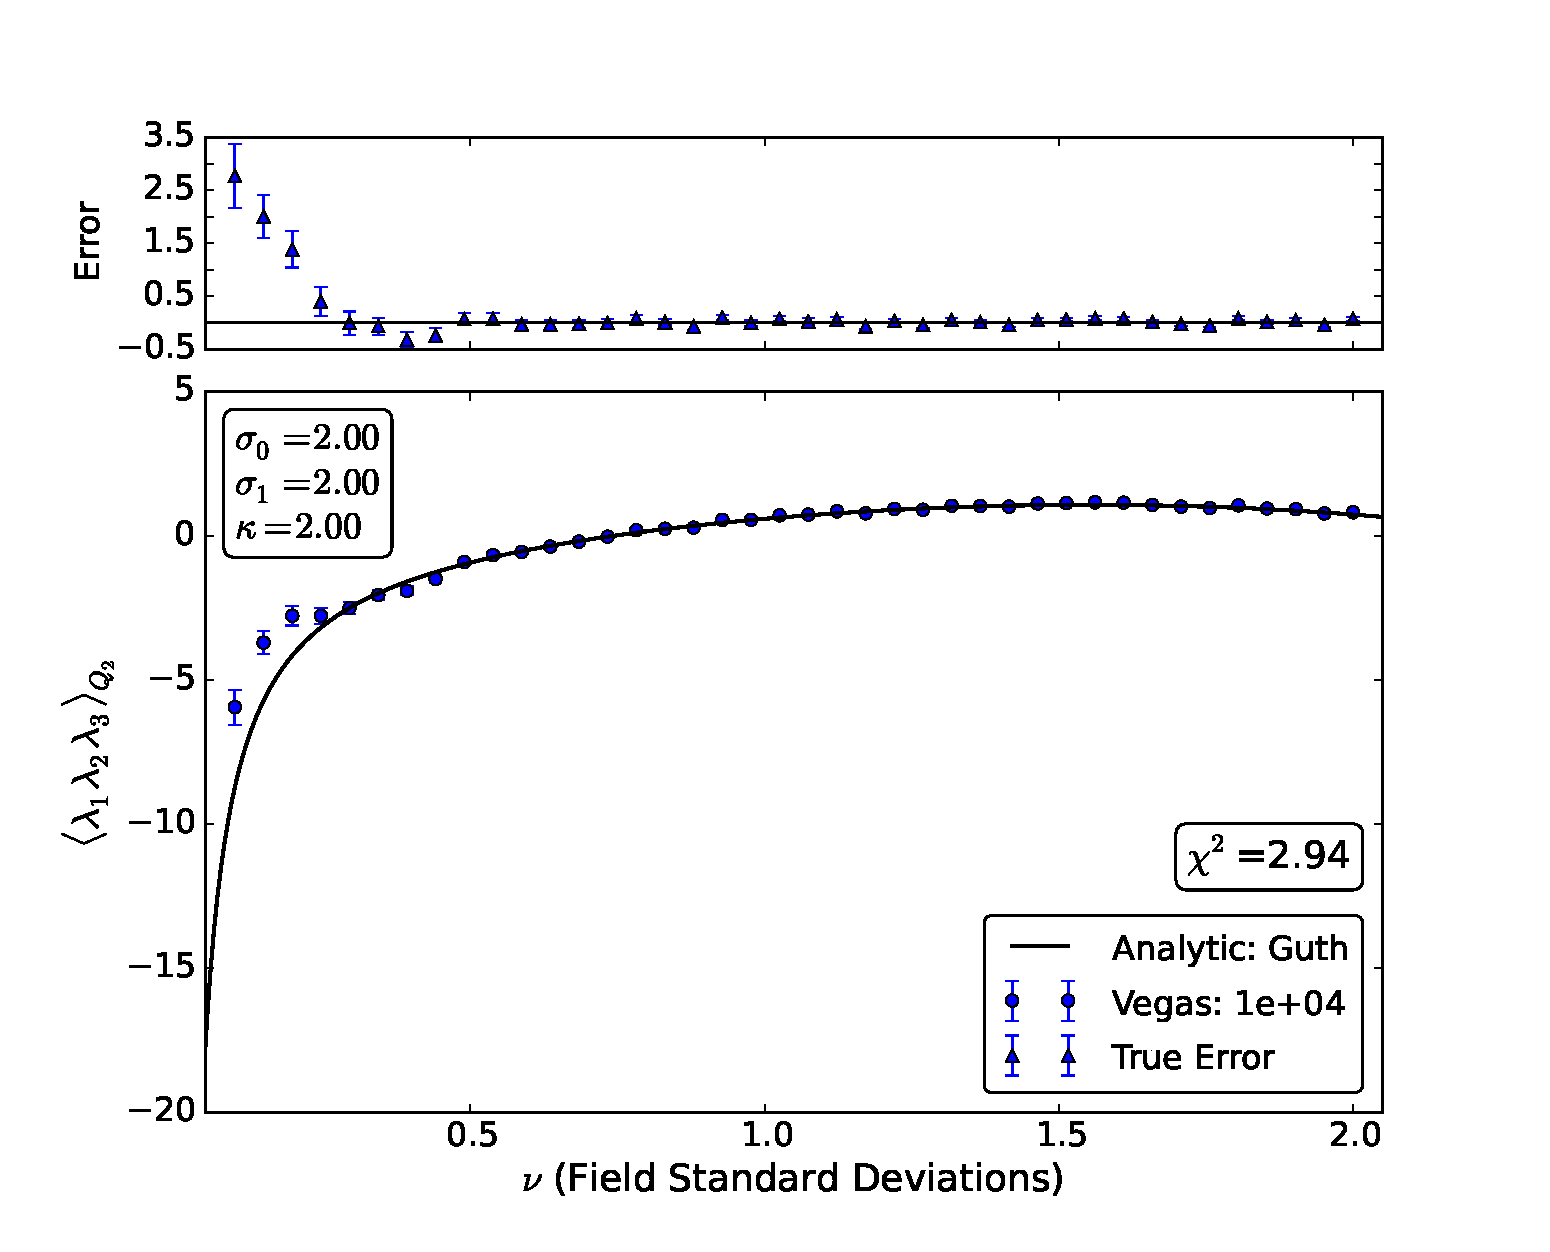
\includegraphics[scale=0.45]{images/toy_int_e4_wide.eps} 
\caption{Test integrations of the toy integral (\ref{eq:toyint}) and its analytic value at varying field heights. $10^4$ samples per iteration.}
\label{fig:toy_e4_wide}
\end{figure}

\begin{figure}[t] %The capital H inside the square brackets is what forces the image to go exactly where I've placed in in the text. You need to be using the float package for this to work. 
\centering %I've put the centering command here so that the image appears centered on the page. 
\includegraphics[scale=0.45]{images/toy_int_e5_wide.eps} 
\caption{Test integrations of the toy integral (\ref{eq:toyint}) and its analytic value at varying field heights. $10^5$ samples per iteration.}
\label{fig:toy_e5_wide}
\end{figure}

\begin{figure}[t] %The capital H inside the square brackets is what forces the image to go exactly where I've placed in in the text. You need to be using the float package for this to work. 
\centering %I've put the centering command here so that the image appears centered on the page. 
\includegraphics[scale=0.45]{images/toy_int_e6_wide.eps} 
\caption{Test integrations of the toy integral (\ref{eq:toyint}) and its analytic value at varying field heights. $10^6$ samples per iteration.}
\label{fig:toy_e6_wide}
\end{figure}

\begin{figure}[t] %The capital H inside the square brackets is what forces the image to go exactly where I've placed in in the text. You need to be using the float package for this to work. 
\centering %I've put the centering command here so that the image appears centered on the page. 
\includegraphics[scale=0.45]{images/toy_pcterr_e4.eps} 
\caption{Test integrations of the toy integral (\ref{eq:toyint}) and its analytic value at varying field heights. $10^6$ samples per iteration.}
\label{fig:toy_pcterr_e4}
\end{figure}

\begin{figure}[t] %The capital H inside the square brackets is what forces the image to go exactly where I've placed in in the text. You need to be using the float package for this to work. 
\centering %I've put the centering command here so that the image appears centered on the page. 
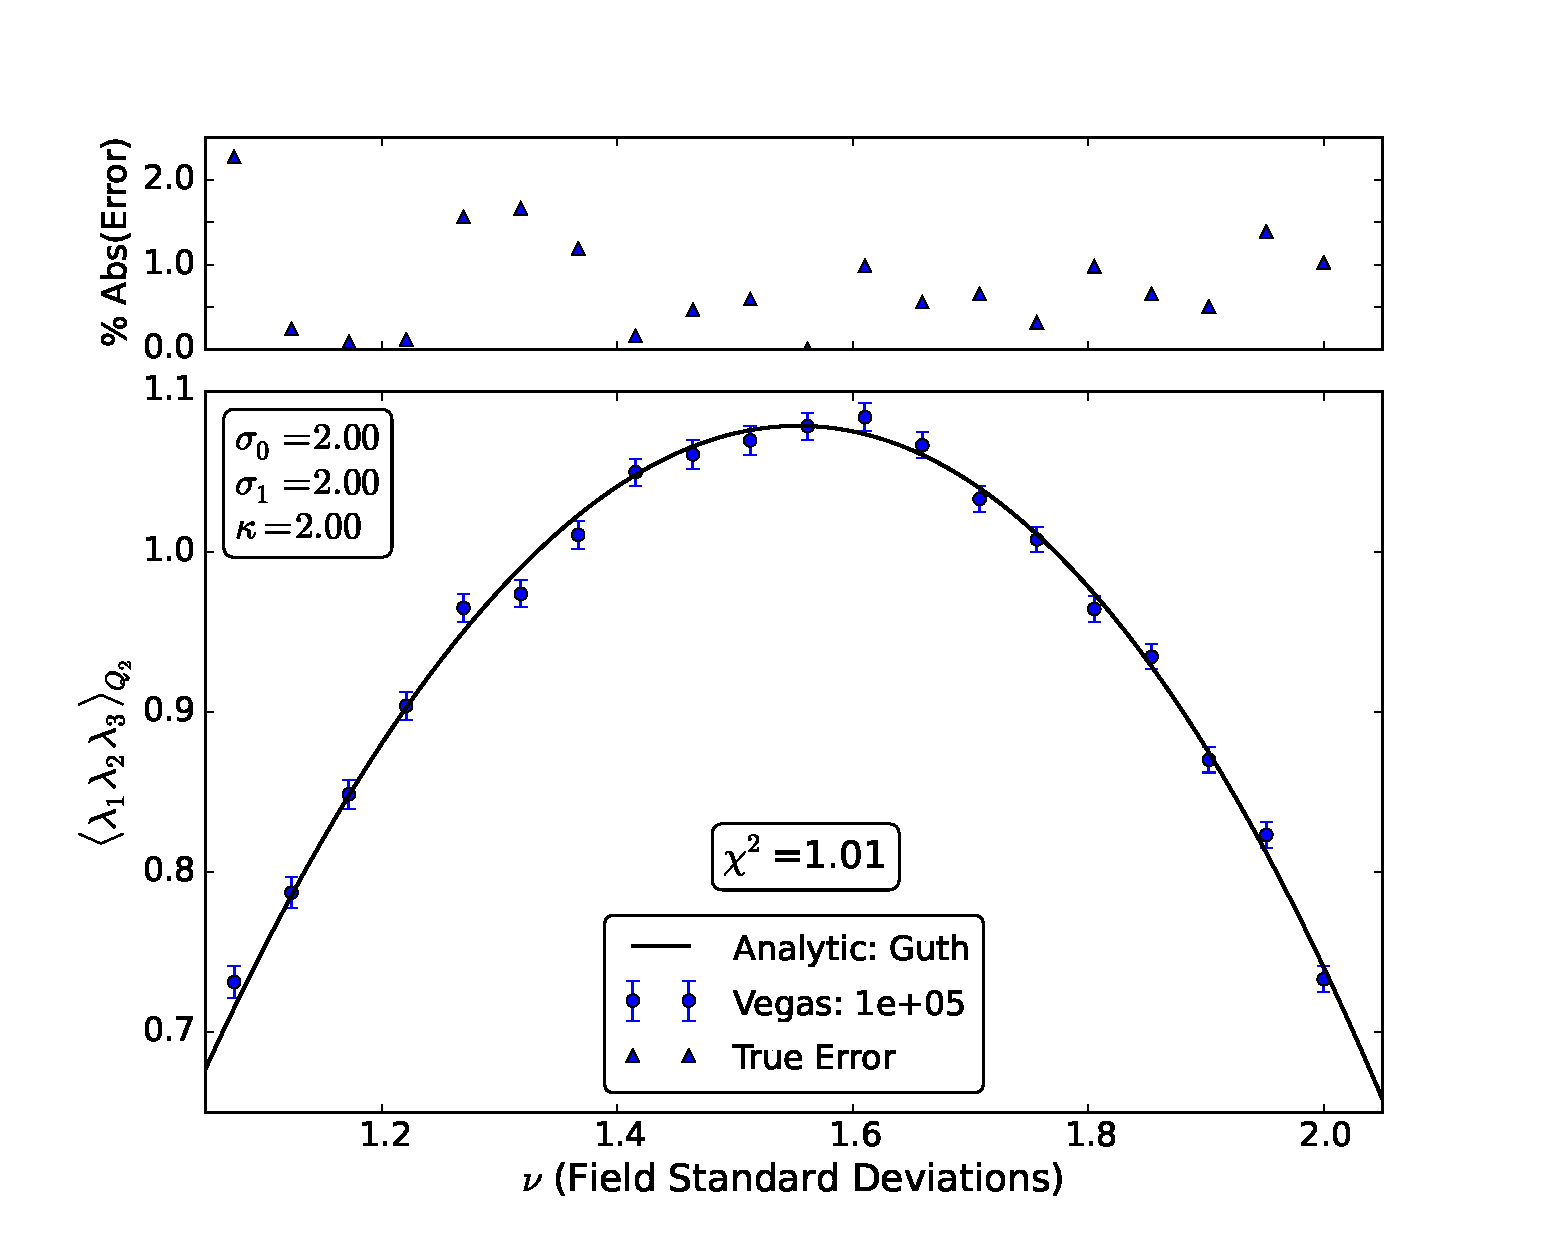
\includegraphics[scale=0.45]{images/toy_pcterr_e5.eps} 
\caption{Test integrations of the toy integral (\ref{eq:toyint}) and its analytic value at varying field heights. $10^6$ samples per iteration.}
\label{fig:toy_pcterr_e5}
\end{figure}

\begin{figure}[t] %The capital H inside the square brackets is what forces the image to go exactly where I've placed in in the text. You need to be using the float package for this to work. 
\centering %I've put the centering command here so that the image appears centered on the page. 
\includegraphics[scale=0.45]{images/toy_pcterr_e6.eps} 
\caption{Test integrations of the toy integral (\ref{eq:toyint}) and its analytic value at varying field heights. $10^6$ samples per iteration.}
\label{fig:toy_pcterr_e6}
\end{figure}


\FloatBarrier

\begin{figure}[t] %The capital H inside the square brackets is what forces the image to go exactly where I've placed in in the text. You need to be using the float package for this to work. 
\centering %I've put the centering command here so that the image appears centered on the page. 
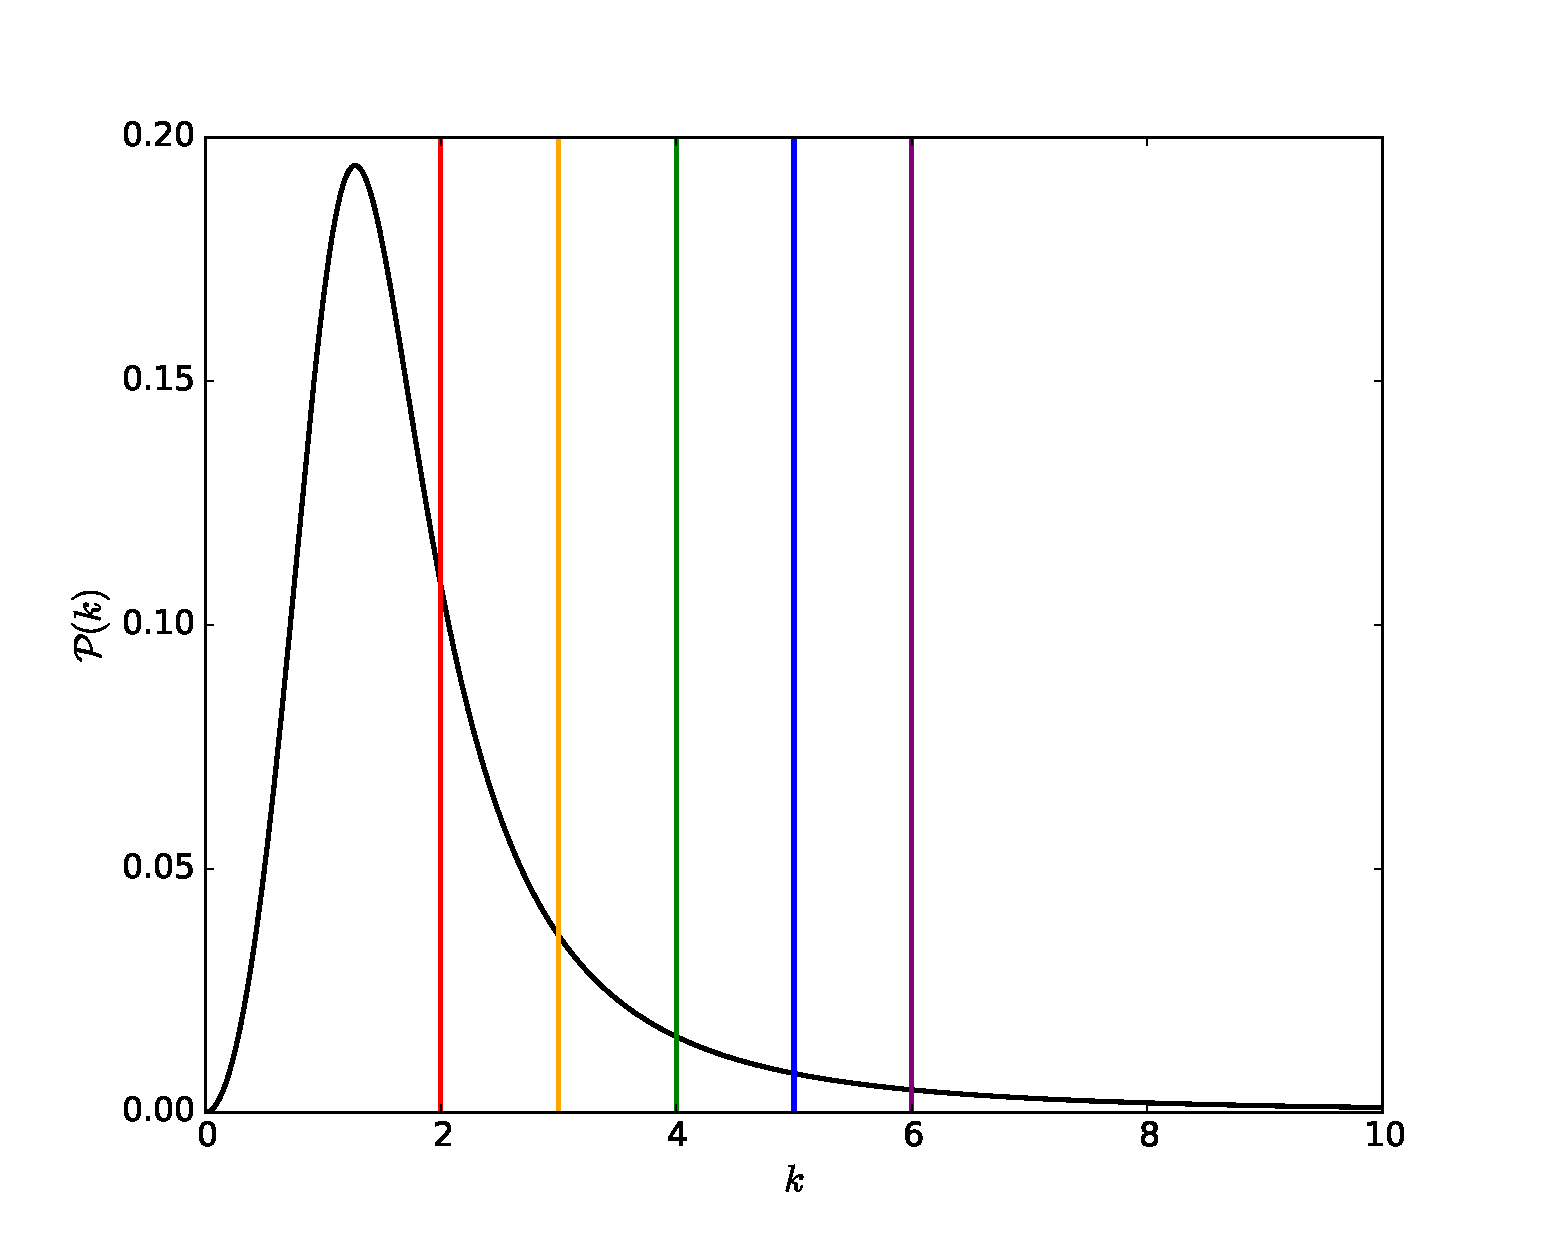
\includegraphics[scale=0.45]{images/cutoff_guide.eps} 
\caption{Test integrations of the toy integral (\ref{eq:toyint}) and its analytic value at varying field heights. $10^6$ samples per iteration.}
\label{fig:toy_e6_wide}
\end{figure}

\begin{figure}[t] %The capital H inside the square brackets is what forces the image to go exactly where I've placed in in the text. You need to be using the float package for this to work. 
\centering %I've put the centering command here so that the image appears centered on the page. 
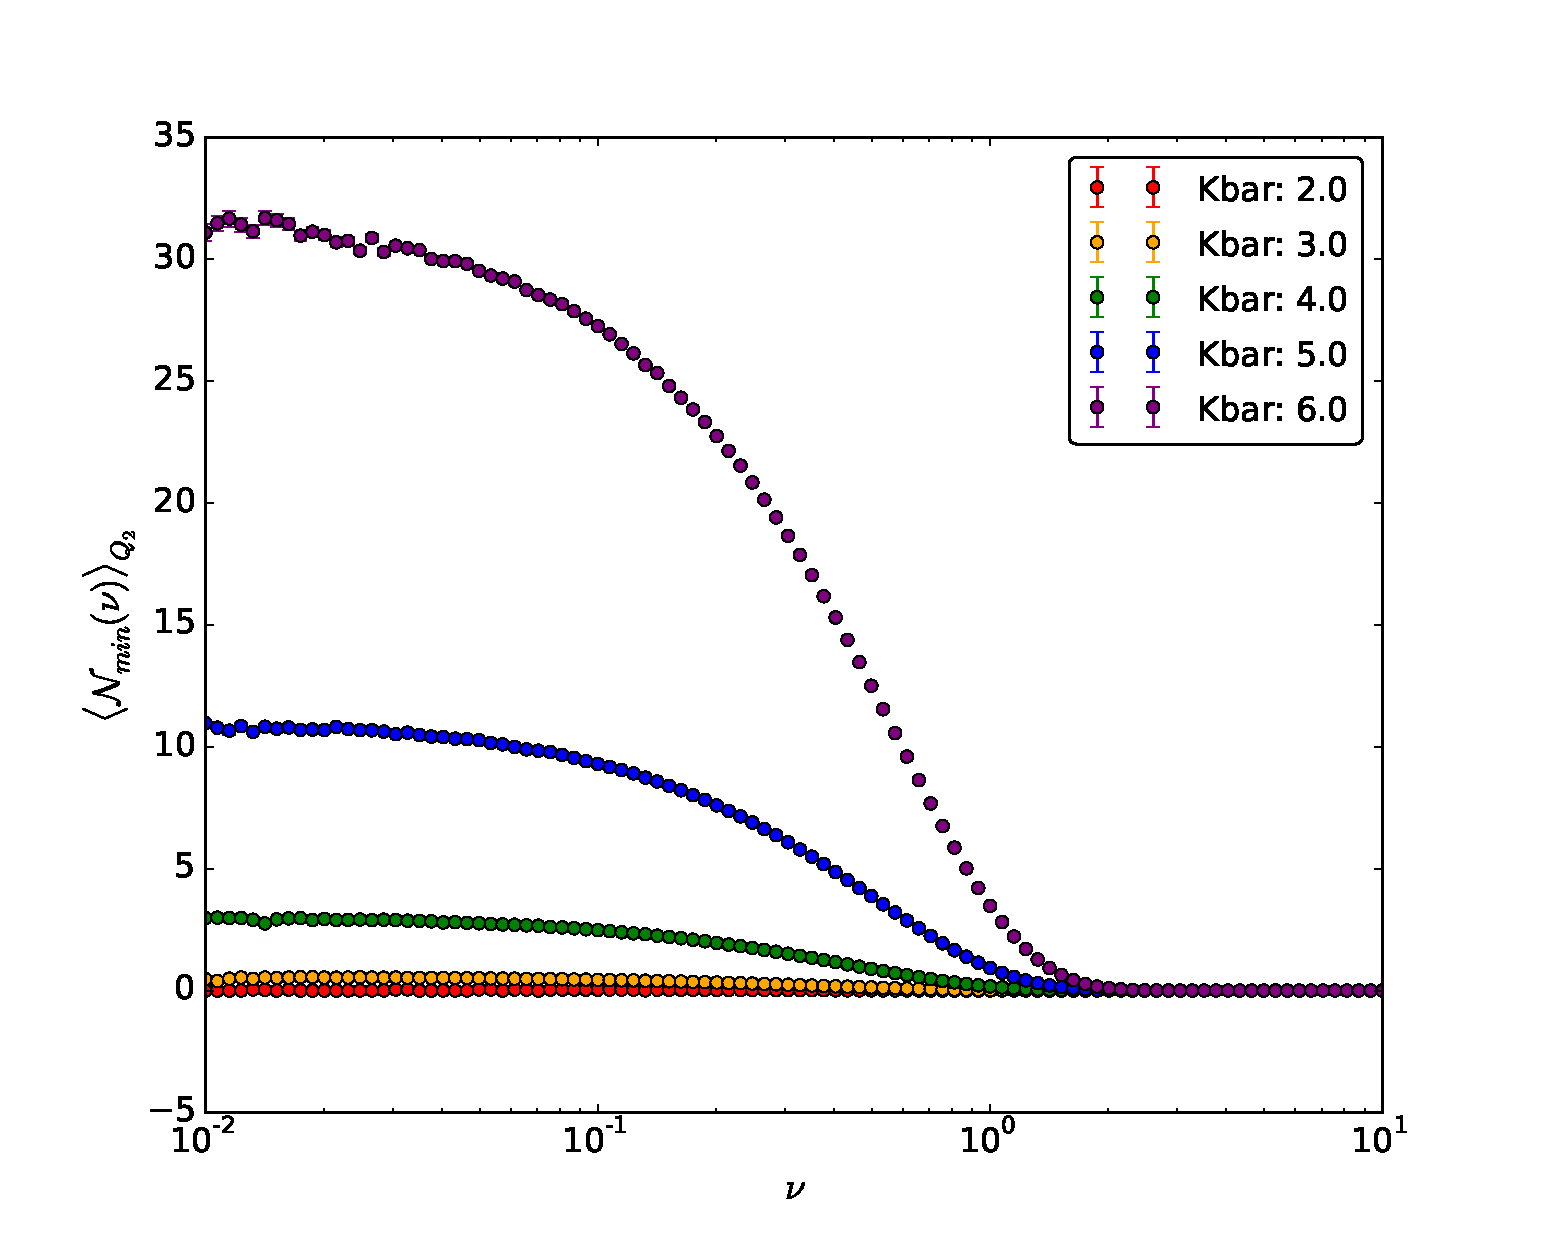
\includegraphics[scale=0.45]{images/density_cutoff_compare_wide.eps} 
\caption{KBAR:  2.0   MAXPCT:  0.00115592612476
KBAR:  3.0   MAXPCT:  0.0117671906972
KBAR:  4.0   MAXPCT:  0.0453885401547
KBAR:  5.0   MAXPCT:  0.166640370797
KBAR:  6.0   MAXPCT:  0.341659925564
}
\label{fig:toy_e6_wide}
\end{figure}

\FloatBarrier

\begin{figure}[t] %The capital H inside the square brackets is what forces the image to go exactly where I've placed in in the text. You need to be using the float package for this to work. 
\centering %I've put the centering command here so that the image appears centered on the page. 
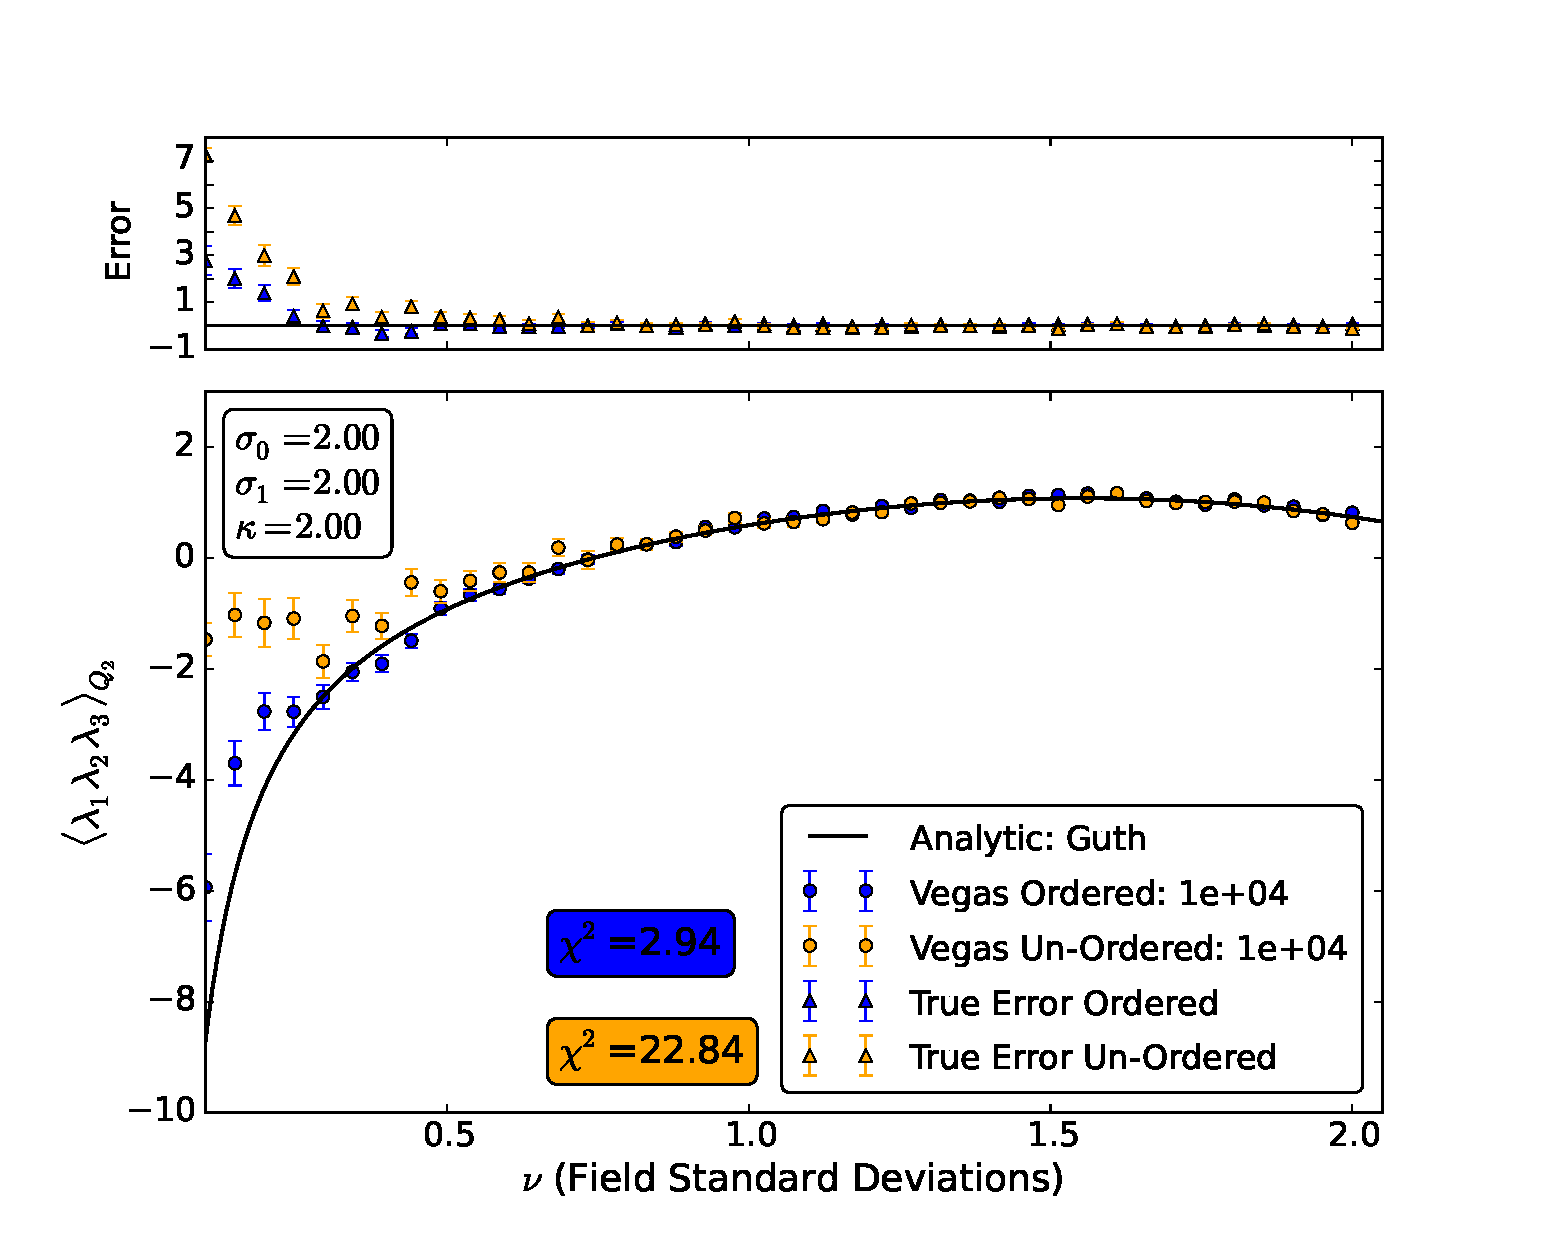
\includegraphics[scale=0.45]{images/ordercomp_e4.eps} 
\caption{Test integrations of the toy integral (\ref{eq:toyint}) and its analytic value at varying field heights. $10^6$ samples per iteration.}
\label{fig:ordercomp_e4}
\end{figure}

\begin{figure}[t] %The capital H inside the square brackets is what forces the image to go exactly where I've placed in in the text. You need to be using the float package for this to work. 
\centering %I've put the centering command here so that the image appears centered on the page. 
\includegraphics[scale=0.45]{images/ordercomp_e5.eps} 
\caption{Test integrations of the toy integral (\ref{eq:toyint}) and its analytic value at varying field heights. $10^6$ samples per iteration.}
\label{fig:ordercomp_e5}
\end{figure}

\begin{figure}[t] %The capital H inside the square brackets is what forces the image to go exactly where I've placed in in the text. You need to be using the float package for this to work. 
\centering %I've put the centering command here so that the image appears centered on the page. 
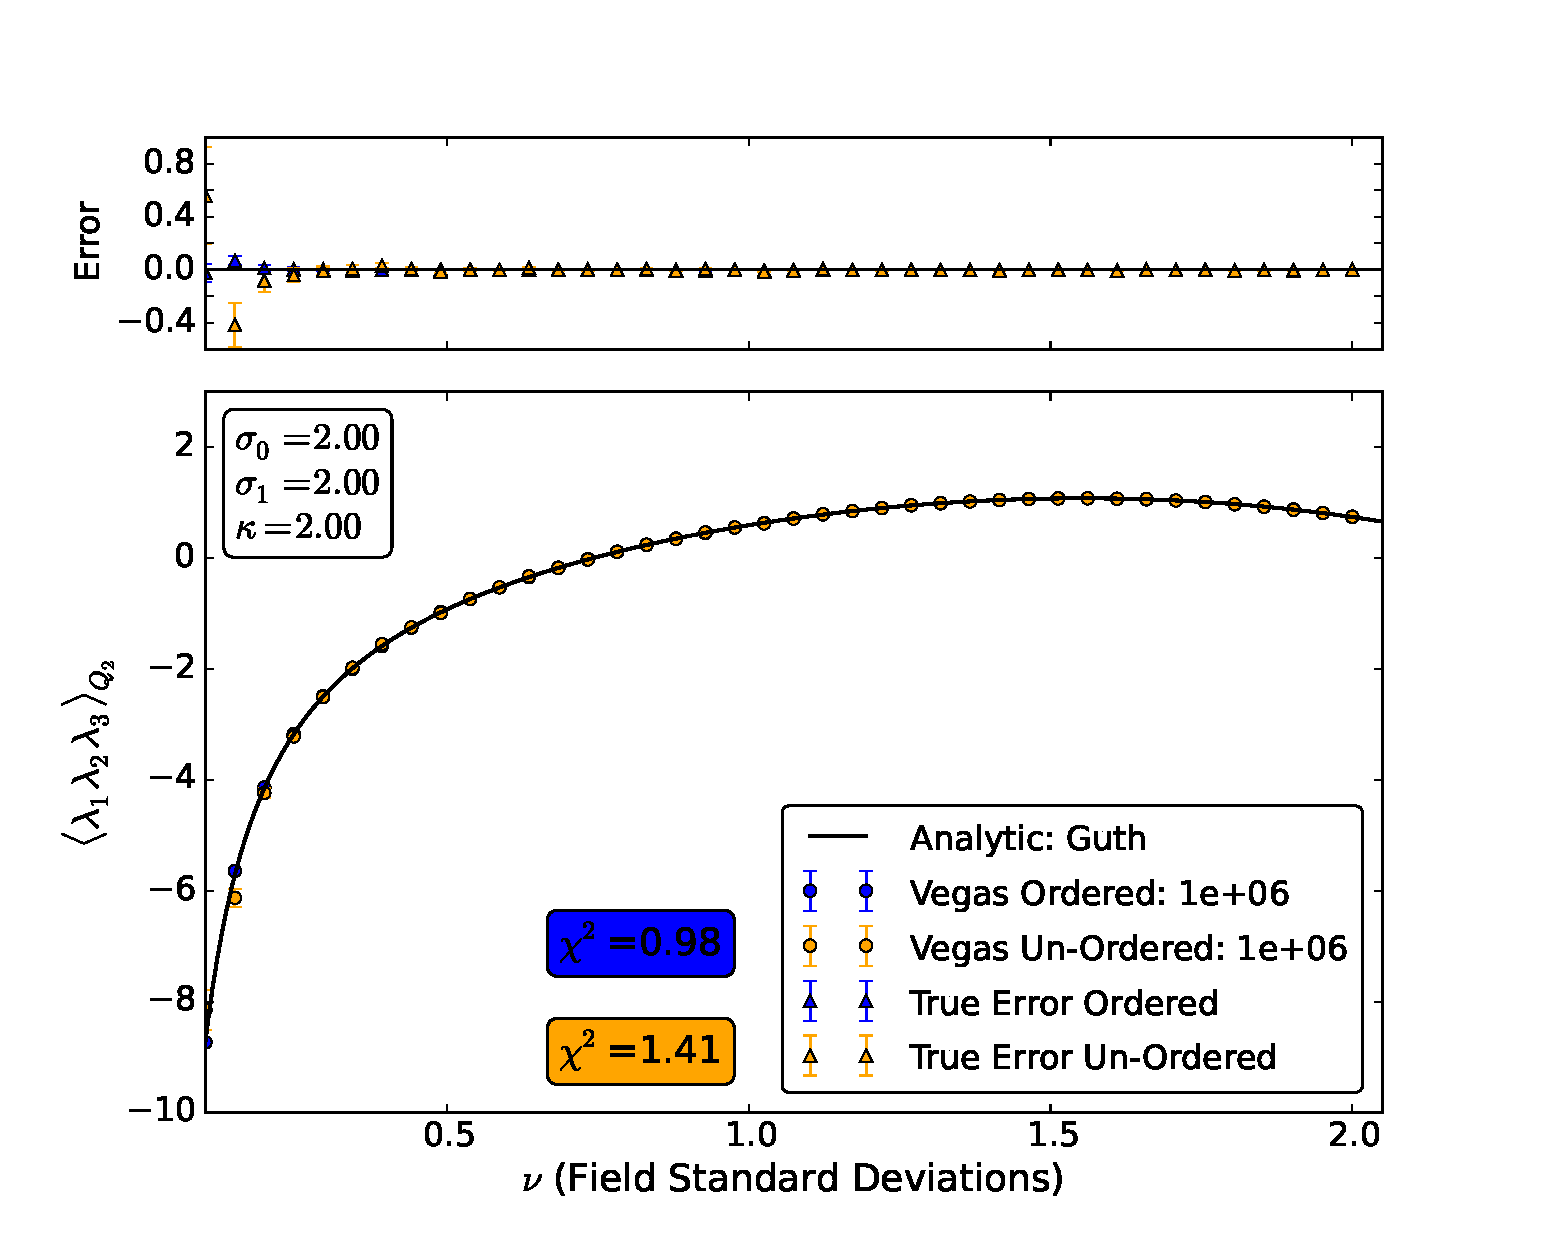
\includegraphics[scale=0.45]{images/ordercomp_e6.eps} 
\caption{Test integrations of the toy integral (\ref{eq:toyint}) and its analytic value at varying field heights. $10^6$ samples per iteration.}
\label{fig:ordercomp_e6}
\end{figure}

\begin{figure}[t] %The capital H inside the square brackets is what forces the image to go exactly where I've placed in in the text. You need to be using the float package for this to work. 
\centering %I've put the centering command here so that the image appears centered on the page. 
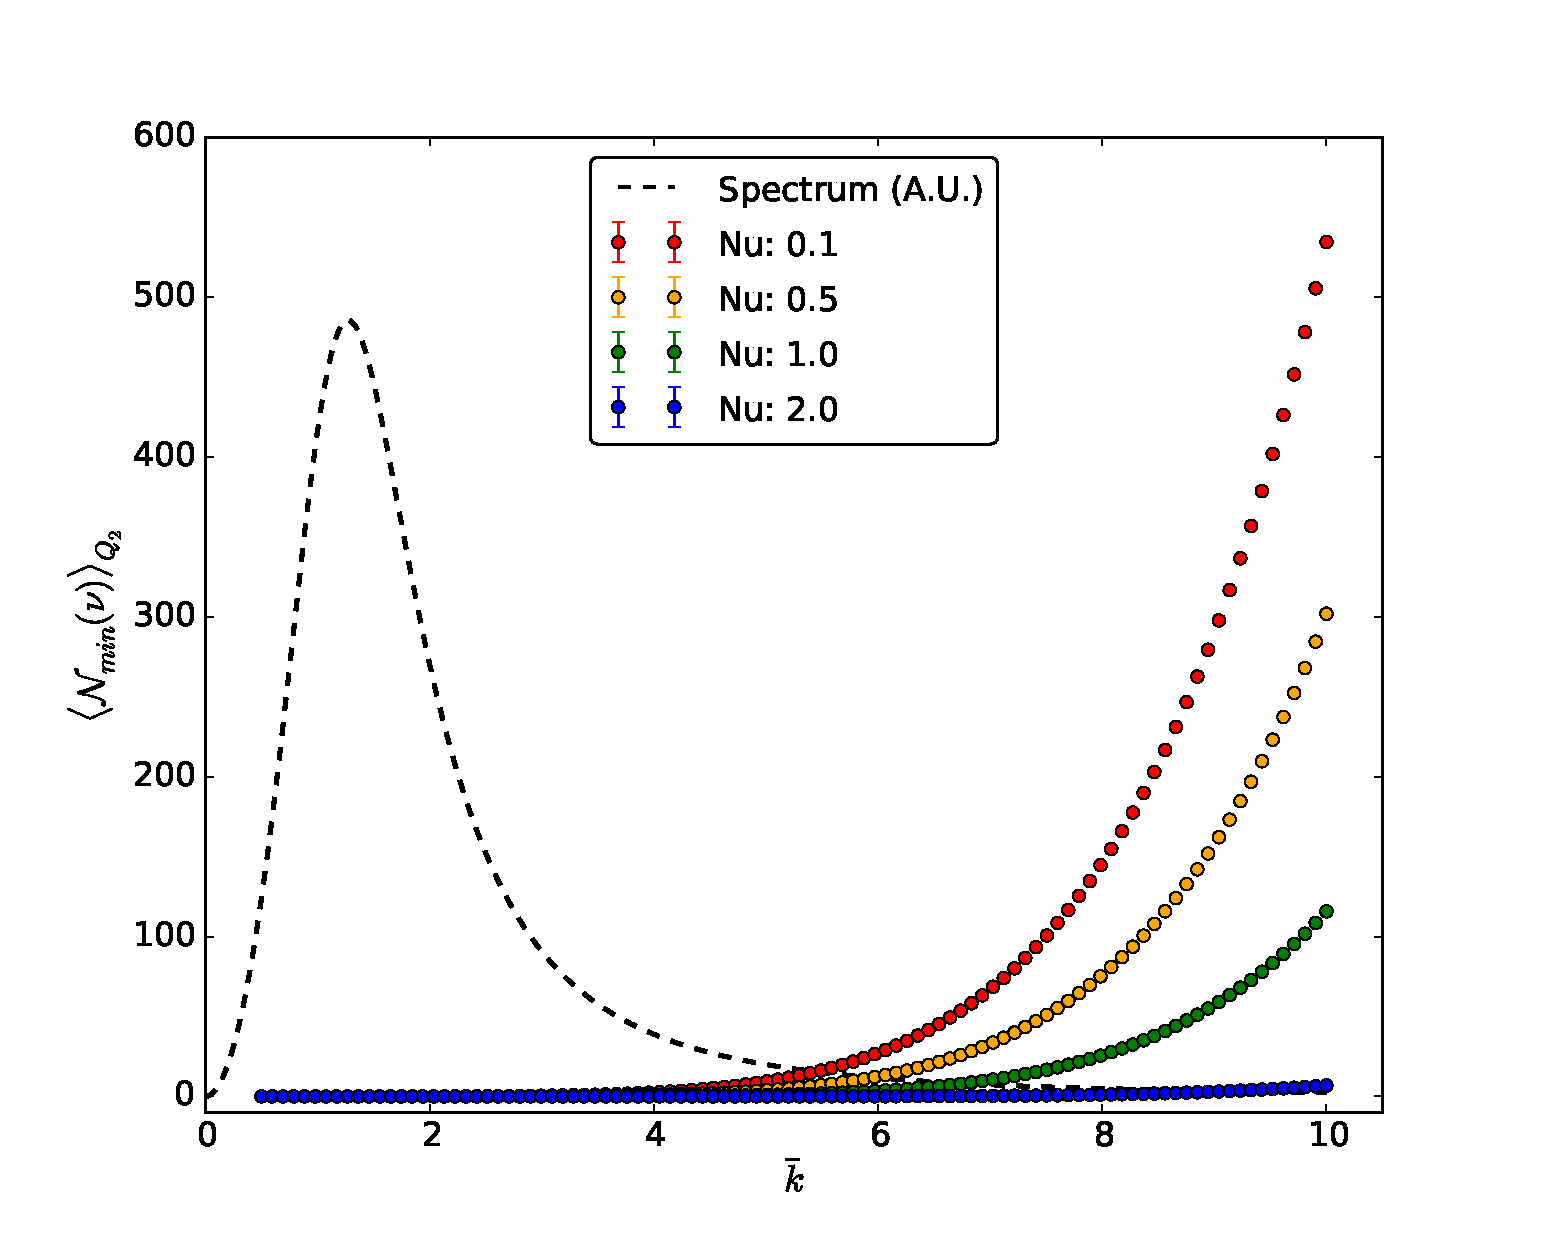
\includegraphics[scale=0.45]{images/spectraplot.eps} 
\caption{Test integrations of the toy integral (\ref{eq:toyint}) and its analytic value at varying field heights. $10^6$ samples per iteration.}
\label{fig:spectraplot}
\end{figure}





%BIB


%@article{doi:10.1137/060661569,
%author = {Pierre Comon and Gene Golub and Lek-Heng Lim and Bernard Mourrain},
%title = {Symmetric Tensors and Symmetric Tensor Rank},
%journal = {SIAM Journal on Matrix Analysis and Applications},
%volume = {30},
%number = {3},
%pages = {1254-1279},
%year = {2008},
%doi = {10.1137/060661569},

%URL = { 
%        http://dx.doi.org/10.1137/060661569
%    
%},
%eprint = { 
%%        http://dx.doi.org/10.1137/060661569
%   
%}%
%
%}




%@article{doi:10.1080/03610918008812164,
%author = {   D. B.   Owen },
%title = {A table of normal integrals},
%journal = {Communications in Statistics - Simulation and Computation},
%volume = {9},
%number = {4},
%pages = {389-419},
%year = {1980},
%doi = {10.1080/03610918008812164},

%URL = { 
%        http://dx.doi.org/10.1080/03610918008812164
%    
%},
%eprint = { 
%        http://dx.doi.org/10.1080/03610918008812164
%    
%}
%
%}




%BIB

%@article{doi:10.1080/03610918008812164,
%author = {   D. B.   Owen },
%title = {A table of normal integrals},
%journal = {Communications in Statistics - Simulation and Computation},
%volume = {9},
%number = {4},
%pages = {389-419},
%year = {1980},
%doi = {10.1080/03610918008812164},

%URL = { 
%        http://dx.doi.org/10.1080/03610918008812164
%    
%},
%eprint = { 
%        http://dx.doi.org/10.1080/03610918008812164
%    
%}
%
%}




\end{document}